\section{Lineare Gleichungssysteme und Matrizen}
\subsection{Grundlagen der Matrizenrechnung}

\subsubsection{Definition Matrix}%
\label{ssub:Definition Matrix}


\begin{equation*}
  A_{m,n} =
  \begin{pmatrix} 
    a_{11} & a_{12} & \cdots & a_{1n} \\
    a_{21} & a_{22} & \cdots & a_{2n} \\
    \vdots  & \vdots  & \ddots & \vdots  \\
    a_{m1} & a_{m2} & \cdots & a_{mn} 
  \end{pmatrix} 
\end{equation*}

Weil die Matrix $m$ Zeilen und $n$ Spalten hat, nennt man sie $m\times n$ Matrix oder $(m,n)$-Matrix.
Merke: Zeile zuerst, Spalte später!

\subsubsection{Addition und Subtraktion}%
\label{ssub:Addition und Subtraktion}
Zwei Matrizen der gleichen Grösse können addiert und subtrahiert werden. Diese Operationen werden \textit{elementweise} durchgeführt, d.h. es werden einfach die entsprechenden Elemente addiert bzw. subtrahiert:
\begin{equation*}
  \begin{pmatrix} 
    1 & 2 \\
    3 & 4
  \end{pmatrix} 
  +
  \begin{pmatrix} 
    5 & 6 \\
    7 & 8
  \end{pmatrix} 
  =
  \begin{pmatrix} 
    1+5 & 2+6 \\
    3+7 & 4+8 
  \end{pmatrix} 
  =
  \begin{pmatrix} 
    6 & 8 \\
    10 & 12 
  \end{pmatrix} 
\end{equation*}

\subsubsection{Skalare Multiplikation}%
\label{ssub:Skalare Multiplikation}
Matrizen können elementweise mit einem Skalar (einer reellen Zahl) multipliziert werden:
\begin{equation*}
  5 \cdot
  \begin{pmatrix} 
    1 & 2 \\
    3 & 4
  \end{pmatrix} 
  =
  \begin{pmatrix} 
    5 \cdot 1 & 5 \cdot 2 \\
    5 \cdot 3 & 5 \cdot 4
  \end{pmatrix} 
  =
  \begin{pmatrix} 
    5 & 10 \\
    15 & 20
  \end{pmatrix} 
\end{equation*}

\subsubsection{Multiplikation}%
\label{ssub:Multiplikation}
Die Multiplikation von Matrizen ist \textit{nicht} elementweise definiert! \\
Damit zwei Matrizen $A$ und $B$ miteinander multipliziert werden können, muss gelten: Die Anzahl Spalten von A ist gleich der Anzahl Zeilen von $B$.
Das Ergebnis hat gleich viele Zeilen wie $A$ und gleich viele Spalten wie $B$.
\begin{center}
  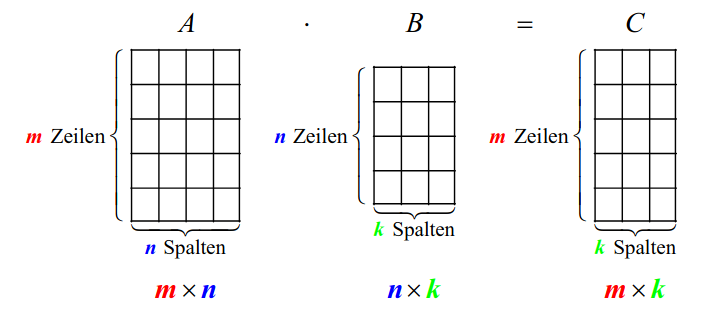
\includegraphics[width=0.6\linewidth]{images/multiplikation.png}
\end{center}
Das Element $c_{ij}$ der $i$-ten Zeile und $j$-ten Spalte der Ergebnismatrix $C$ wird so berechnet:
\begin{center}
  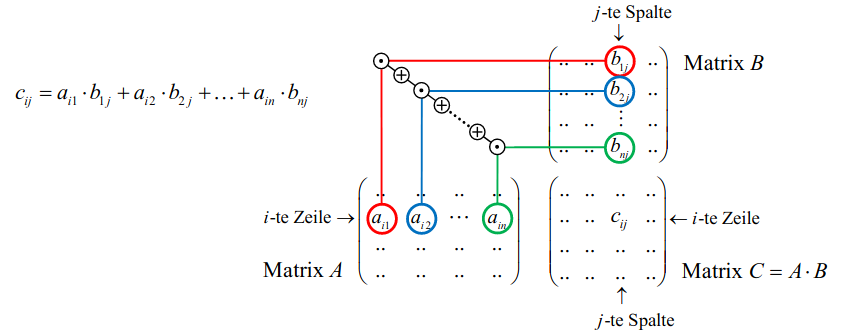
\includegraphics[width=0.8\linewidth]{images/multiplikation2.png}
\end{center}

\vfill

\subsubsection{Transponierte}%
\label{ssub:Transponierte}
Die Transponierte einer $m \times n$-Matrix ist eine $n \times m$-Matrix. Man erhält diese, indem man die Zeilen zu Spalten macht (und umgekehrt):
\begin{center}
  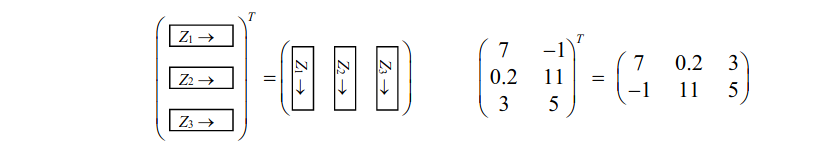
\includegraphics[width=0.8\linewidth]{images/transponierte.png}
\end{center}

\subsubsection{Rechenregeln für Addition und skalare Multiplikation}%
\label{ssub:Rechenregeln für Addition und skalare Multiplikation}
Für beliebige $m \times n$-Matrizen $A$ und $B$ sowie für einen beliebigen Skalar $\lambda \in \mathbb{R}$ gilt:
\begin{enumerate}
  \item \textit{Kommutativ-Gesetz: } $A+B=B+A$
  \item \textit{Assoziativ-Gesetz: } $A+(B+C)=(A+B)+C$
  \item \textit{Distributiv-Gesetz: } $\lambda \cdot (A+B) = \lambda \cdot A + \lambda \cdot B$ und $(\lambda + \mu) \cdot A = \lambda \cdot A + \mu \cdot A$
\end{enumerate}

\subsubsection{Rechenregeln für Multiplikation}%
\label{ssub:Rechenregeln für Multiplikation}
Für beliebige Matrizen $A,B$ und $C$ von geeigneten Typ sowie für einen beliebigen Skalar $\lambda$ gilt:
\begin{enumerate}
  \item \textit{Assoziativ-Gesetz: } $A \cdot (B \cdot C)=(A \cdot B) \cdot C$
  \item \textit{Distributiv-Gesetz: } $A \cdot (B+C) = A \cdot B + A \cdot C$ und $(A+B) \cdot C = A \cdot C = A \cdot C + B \cdot C$
  \item \textit{Regel zur Multiplikation mit einem Skalar: } $(\lambda \cdot A) \cdot B = \lambda \cdot (A \cdot B) = A \cdot (\lambda \cdot B)$
\end{enumerate}
\textbf{Die Matrizenmultiplikation ist nicht kommutativ!!!} \\
Im Allgemeinen gilt: $A \cdot B \neq B \cdot A$!

\subsection{Lineare Gleichungssysteme LGS}
Jedes LGS entspricht einer Matrizengleichung:
\begin{center}
  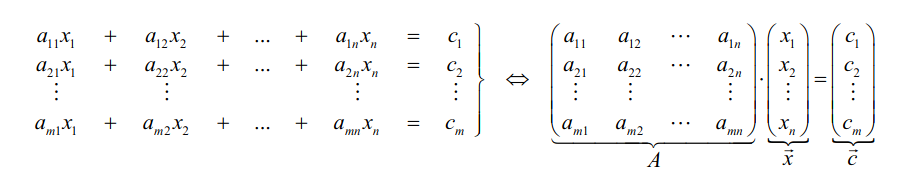
\includegraphics[width=0.9\linewidth]{images/lgs.png}
\end{center}
Wir fassen $A$ und $\vec{c}$ zur \textit{erweiterten Koeffizientenmatrix} zusammen:
\begin{equation*}
  (A|\vec{c})=
  \begin{pmatrix}[cccc|c]
    a_{11} & a_{12} & \cdots & a_{1n} & c_1 \\
    a_{21} & a_{22} & \cdots & a_{2n} & c_2 \\
    \vdots & \vdots & \ddots & \vdots & \vdots \\
    a_{m1} & a_{m2} & \cdots & a_{mn} & c_m
  \end{pmatrix} 
\end{equation*}

\subsubsection{Gauss-Jordan-Verfahren}%
\label{ssub:Gauss-Jordan-Verfahren}
\begin{enumerate}
  \item Wir bestimmen die am weitesten links stehende Spalte mit Elementen $\neq 0$. Wir nennen diese Spalte die \textit{Pivot-Spalte}.
  \item Ist die oberste Zahl in der Pivot-Spalte $=0$, dann vertauschen wir die erste Zeile mit der obersten Zeile, die in der Pivot-Spalte ein Element $\neq 0$ hat.
  \item Die oberste Zahl in der Pivot-Spalte ist nun eine Zahl $a \neq 0$. Wir dividieren die erste Zeile durch $a$. So erhalten wir die führende Eins.
  \item Nun wollen wir unterhalb der führenden Eins lauter Nullen erzeugen. Dazu addieren wir passende Vielfache der ersten Zeile zu den übrigen Zeilen.
    Wir lassen nun die erste Zeile aussen vor und wenden die ersten vier Schritte auf den verbleibenden Teil der Matrix an. Dieses Verfahren wiederholen wir so oft, bis die erweiterte Koeffizientenmatrix Zeilenstufenform hat.
  \item Nun arbeiten wir von unten nach oben und addieren jeweils geeignete Vielfache jeder Zeile zu den darüber liegenden Zeilen, um über den führenden Einsen Nullen zu erzeugen.
\end{enumerate}

Das Gauss-Jordan-Verfahren bringt die erweiterte Koeffizientenmatrix auf \textit{reduzierte Zeilenstufenform}, d.h.
\begin{itemize}
  \item Alle Zeilen, die nur Nullen enthalten, stehen zuunterst (falls vorhanden).
  \item Wenn eine Zeile nicht nur aus Nullen besteht, so ist die vorderste Zahl $\neq 0$ eine Eins. Sie wird als \textit{führende Eins} der Zeile bezeichnet.
  \item Eine führende Eins, die weiter unten als eine andere führende Eins steht, steht auch weiter rechts.
  \item Jede Spalte, in der eine führende Eins steht, enthält sonst nur Nullen.
\end{itemize}

\subsubsection{Bestimmung der Lösungen eines LGS aus der reduzierten Zeilenstufenform}%
\label{ssub:Bestimmung der Lösungen eines LGS aus der reduzierten Zeilenstufenform}
Wir ordnen den Spalten der Koeffizientenmatrix die entsprechenden Unbekannten zu. Unbekannte, die zu einer Spalte \textbf{mit} führender Eins gehören, heissen \textit{führende Unbekannte}. Unbekannte, die zu einer Spalte \textbf{ohne} führender Eins gehören, heissen \textit{freie Unbekannte}.
\begin{center}
  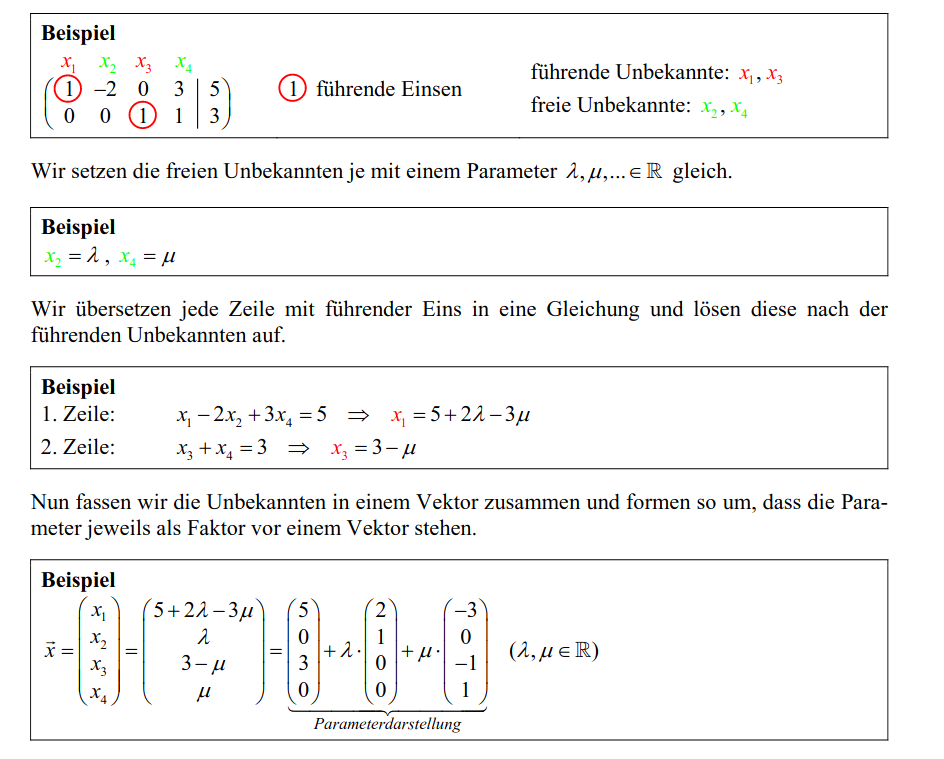
\includegraphics[width=0.8\linewidth]{images/lgs_zsf.png}
\end{center}

\subsubsection{Rang}%
\label{ssub:Rang}
$rg(A)=$ Gesamtanzahl Zeilen - Anzahl Nullzeilen (Wenn Matrix $A$ auf ZSF).

\subsubsection{Kriterien für die Anzahl Lösungen eines LGS}%
\label{ssub:Kriterien für die Anzahl Lösungen eines LGS}
\begin{center}
  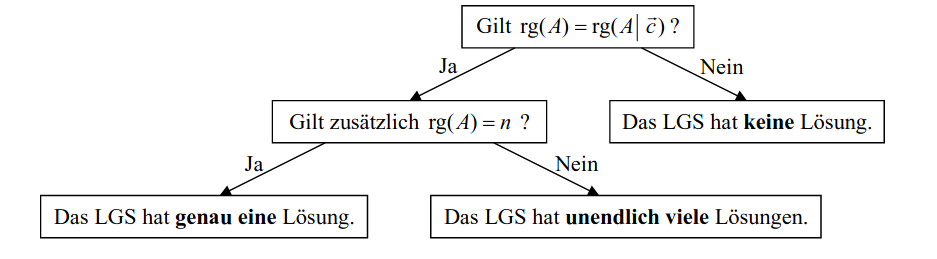
\includegraphics[width=0.8\linewidth]{images/kriterien.png}
\end{center}


